% Created by tikzDevice version 0.7.0 on 2014-06-17 19:18:57
% !TEX encoding = UTF-8 Unicode
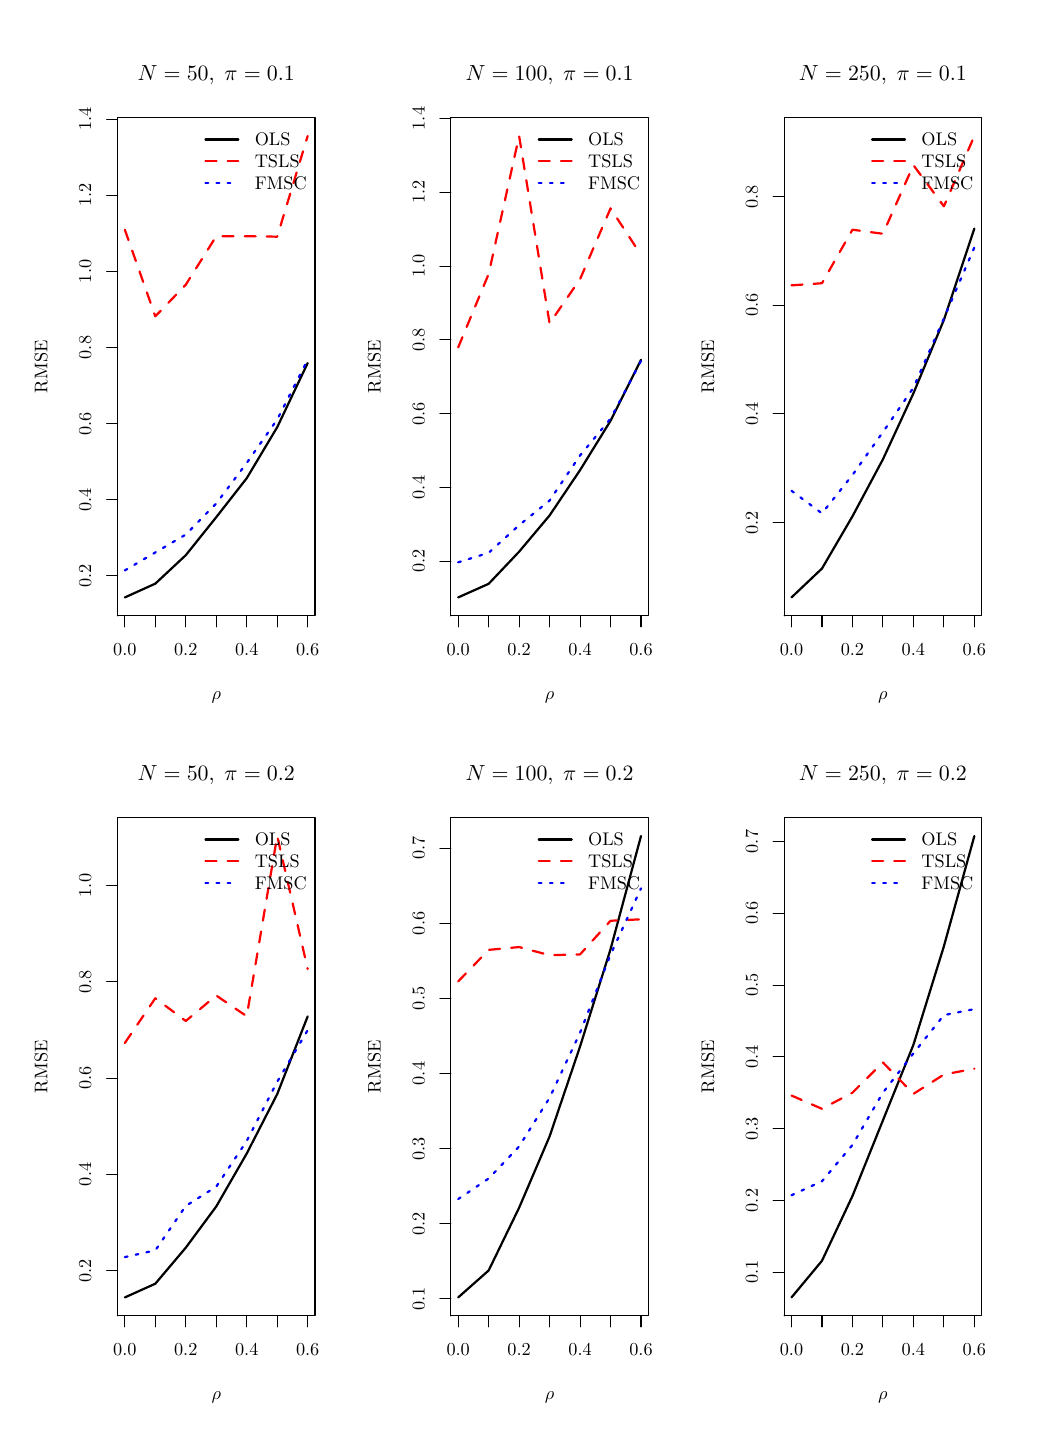
\begin{tikzpicture}[x=1pt,y=1pt]
\definecolor[named]{fillColor}{rgb}{1.00,1.00,1.00}
\path[use as bounding box,fill=fillColor,fill opacity=0.00] (0,0) rectangle (361.35,505.89);
\begin{scope}
\path[clip] ( 32.47,293.34) rectangle (103.82,473.42);
\definecolor[named]{drawColor}{rgb}{0.00,0.00,0.00}

\path[draw=drawColor,line width= 0.8pt,line join=round,line cap=round] ( 35.11,300.01) --
	( 46.12,304.98) --
	( 57.13,315.27) --
	( 68.14,329.00) --
	( 79.16,343.09) --
	( 90.17,361.52) --
	(101.18,384.69);
\end{scope}
\begin{scope}
\path[clip] (  0.00,  0.00) rectangle (361.35,505.89);
\definecolor[named]{drawColor}{rgb}{0.00,0.00,0.00}

\path[draw=drawColor,line width= 0.4pt,line join=round,line cap=round] ( 35.11,293.34) -- (101.18,293.34);

\path[draw=drawColor,line width= 0.4pt,line join=round,line cap=round] ( 35.11,293.34) -- ( 35.11,289.38);

\path[draw=drawColor,line width= 0.4pt,line join=round,line cap=round] ( 46.12,293.34) -- ( 46.12,289.38);

\path[draw=drawColor,line width= 0.4pt,line join=round,line cap=round] ( 57.13,293.34) -- ( 57.13,289.38);

\path[draw=drawColor,line width= 0.4pt,line join=round,line cap=round] ( 68.14,293.34) -- ( 68.14,289.38);

\path[draw=drawColor,line width= 0.4pt,line join=round,line cap=round] ( 79.16,293.34) -- ( 79.16,289.38);

\path[draw=drawColor,line width= 0.4pt,line join=round,line cap=round] ( 90.17,293.34) -- ( 90.17,289.38);

\path[draw=drawColor,line width= 0.4pt,line join=round,line cap=round] (101.18,293.34) -- (101.18,289.38);

\node[text=drawColor,anchor=base,inner sep=0pt, outer sep=0pt, scale=  0.66] at ( 35.11,279.08) {0.0};

\node[text=drawColor,anchor=base,inner sep=0pt, outer sep=0pt, scale=  0.66] at ( 57.13,279.08) {0.2};

\node[text=drawColor,anchor=base,inner sep=0pt, outer sep=0pt, scale=  0.66] at ( 79.16,279.08) {0.4};

\node[text=drawColor,anchor=base,inner sep=0pt, outer sep=0pt, scale=  0.66] at (101.18,279.08) {0.6};

\path[draw=drawColor,line width= 0.4pt,line join=round,line cap=round] ( 32.47,307.78) -- ( 32.47,472.86);

\path[draw=drawColor,line width= 0.4pt,line join=round,line cap=round] ( 32.47,307.78) -- ( 28.51,307.78);

\path[draw=drawColor,line width= 0.4pt,line join=round,line cap=round] ( 32.47,335.30) -- ( 28.51,335.30);

\path[draw=drawColor,line width= 0.4pt,line join=round,line cap=round] ( 32.47,362.81) -- ( 28.51,362.81);

\path[draw=drawColor,line width= 0.4pt,line join=round,line cap=round] ( 32.47,390.32) -- ( 28.51,390.32);

\path[draw=drawColor,line width= 0.4pt,line join=round,line cap=round] ( 32.47,417.84) -- ( 28.51,417.84);

\path[draw=drawColor,line width= 0.4pt,line join=round,line cap=round] ( 32.47,445.35) -- ( 28.51,445.35);

\path[draw=drawColor,line width= 0.4pt,line join=round,line cap=round] ( 32.47,472.86) -- ( 28.51,472.86);

\node[text=drawColor,rotate= 90.00,anchor=base,inner sep=0pt, outer sep=0pt, scale=  0.66] at ( 22.97,307.78) {0.2};

\node[text=drawColor,rotate= 90.00,anchor=base,inner sep=0pt, outer sep=0pt, scale=  0.66] at ( 22.97,335.30) {0.4};

\node[text=drawColor,rotate= 90.00,anchor=base,inner sep=0pt, outer sep=0pt, scale=  0.66] at ( 22.97,362.81) {0.6};

\node[text=drawColor,rotate= 90.00,anchor=base,inner sep=0pt, outer sep=0pt, scale=  0.66] at ( 22.97,390.32) {0.8};

\node[text=drawColor,rotate= 90.00,anchor=base,inner sep=0pt, outer sep=0pt, scale=  0.66] at ( 22.97,417.84) {1.0};

\node[text=drawColor,rotate= 90.00,anchor=base,inner sep=0pt, outer sep=0pt, scale=  0.66] at ( 22.97,445.35) {1.2};

\node[text=drawColor,rotate= 90.00,anchor=base,inner sep=0pt, outer sep=0pt, scale=  0.66] at ( 22.97,472.86) {1.4};

\path[draw=drawColor,line width= 0.4pt,line join=round,line cap=round] ( 32.47,293.34) --
	(103.82,293.34) --
	(103.82,473.42) --
	( 32.47,473.42) --
	( 32.47,293.34);
\end{scope}
\begin{scope}
\path[clip] (  0.00,252.94) rectangle (120.45,505.89);
\definecolor[named]{drawColor}{rgb}{0.00,0.00,0.00}

\node[text=drawColor,anchor=base,inner sep=0pt, outer sep=0pt, scale=  0.79] at ( 68.14,486.92) {\bfseries $N=50, \;\pi=0.1$};

\node[text=drawColor,anchor=base,inner sep=0pt, outer sep=0pt, scale=  0.66] at ( 68.14,263.24) {$\rho$};

\node[text=drawColor,rotate= 90.00,anchor=base,inner sep=0pt, outer sep=0pt, scale=  0.66] at (  7.13,383.38) {RMSE};
\end{scope}
\begin{scope}
\path[clip] ( 32.47,293.34) rectangle (103.82,473.42);
\definecolor[named]{drawColor}{rgb}{1.00,0.00,0.00}

\path[draw=drawColor,line width= 0.8pt,dash pattern=on 4pt off 4pt ,line join=round,line cap=round] ( 35.11,432.88) --
	( 46.12,401.58) --
	( 57.13,413.00) --
	( 68.14,430.53) --
	( 79.16,430.52) --
	( 90.17,430.36) --
	(101.18,466.75);
\definecolor[named]{drawColor}{rgb}{0.00,0.00,1.00}

\path[draw=drawColor,line width= 0.8pt,dash pattern=on 1pt off 3pt ,line join=round,line cap=round] ( 35.11,309.76) --
	( 46.12,316.26) --
	( 57.13,322.72) --
	( 68.14,333.95) --
	( 79.16,348.60) --
	( 90.17,364.31) --
	(101.18,385.84);
\definecolor[named]{drawColor}{rgb}{0.00,0.00,0.00}

\path[draw=drawColor,line width= 0.8pt,line join=round,line cap=round] ( 64.24,465.50) -- ( 76.12,465.50);
\definecolor[named]{drawColor}{rgb}{1.00,0.00,0.00}

\path[draw=drawColor,line width= 0.8pt,dash pattern=on 4pt off 4pt ,line join=round,line cap=round] ( 64.24,457.58) -- ( 76.12,457.58);
\definecolor[named]{drawColor}{rgb}{0.00,0.00,1.00}

\path[draw=drawColor,line width= 0.8pt,dash pattern=on 1pt off 3pt ,line join=round,line cap=round] ( 64.24,449.66) -- ( 76.12,449.66);
\definecolor[named]{drawColor}{rgb}{0.00,0.00,0.00}

\node[text=drawColor,anchor=base west,inner sep=0pt, outer sep=0pt, scale=  0.66] at ( 82.06,463.23) {OLS};

\node[text=drawColor,anchor=base west,inner sep=0pt, outer sep=0pt, scale=  0.66] at ( 82.06,455.31) {TSLS};

\node[text=drawColor,anchor=base west,inner sep=0pt, outer sep=0pt, scale=  0.66] at ( 82.06,447.39) {FMSC};
\end{scope}
\begin{scope}
\path[clip] ( 32.47, 40.39) rectangle (103.82,220.47);
\definecolor[named]{drawColor}{rgb}{0.00,0.00,0.00}

\path[draw=drawColor,line width= 0.8pt,line join=round,line cap=round] ( 35.11, 47.06) --
	( 46.12, 52.02) --
	( 57.13, 65.04) --
	( 68.14, 79.93) --
	( 79.16, 99.07) --
	( 90.17,120.53) --
	(101.18,148.61);
\end{scope}
\begin{scope}
\path[clip] (  0.00,  0.00) rectangle (361.35,505.89);
\definecolor[named]{drawColor}{rgb}{0.00,0.00,0.00}

\path[draw=drawColor,line width= 0.4pt,line join=round,line cap=round] ( 35.11, 40.39) -- (101.18, 40.39);

\path[draw=drawColor,line width= 0.4pt,line join=round,line cap=round] ( 35.11, 40.39) -- ( 35.11, 36.43);

\path[draw=drawColor,line width= 0.4pt,line join=round,line cap=round] ( 46.12, 40.39) -- ( 46.12, 36.43);

\path[draw=drawColor,line width= 0.4pt,line join=round,line cap=round] ( 57.13, 40.39) -- ( 57.13, 36.43);

\path[draw=drawColor,line width= 0.4pt,line join=round,line cap=round] ( 68.14, 40.39) -- ( 68.14, 36.43);

\path[draw=drawColor,line width= 0.4pt,line join=round,line cap=round] ( 79.16, 40.39) -- ( 79.16, 36.43);

\path[draw=drawColor,line width= 0.4pt,line join=round,line cap=round] ( 90.17, 40.39) -- ( 90.17, 36.43);

\path[draw=drawColor,line width= 0.4pt,line join=round,line cap=round] (101.18, 40.39) -- (101.18, 36.43);

\node[text=drawColor,anchor=base,inner sep=0pt, outer sep=0pt, scale=  0.66] at ( 35.11, 26.14) {0.0};

\node[text=drawColor,anchor=base,inner sep=0pt, outer sep=0pt, scale=  0.66] at ( 57.13, 26.14) {0.2};

\node[text=drawColor,anchor=base,inner sep=0pt, outer sep=0pt, scale=  0.66] at ( 79.16, 26.14) {0.4};

\node[text=drawColor,anchor=base,inner sep=0pt, outer sep=0pt, scale=  0.66] at (101.18, 26.14) {0.6};

\path[draw=drawColor,line width= 0.4pt,line join=round,line cap=round] ( 32.47, 56.75) -- ( 32.47,195.91);

\path[draw=drawColor,line width= 0.4pt,line join=round,line cap=round] ( 32.47, 56.75) -- ( 28.51, 56.75);

\path[draw=drawColor,line width= 0.4pt,line join=round,line cap=round] ( 32.47, 91.54) -- ( 28.51, 91.54);

\path[draw=drawColor,line width= 0.4pt,line join=round,line cap=round] ( 32.47,126.33) -- ( 28.51,126.33);

\path[draw=drawColor,line width= 0.4pt,line join=round,line cap=round] ( 32.47,161.12) -- ( 28.51,161.12);

\path[draw=drawColor,line width= 0.4pt,line join=round,line cap=round] ( 32.47,195.91) -- ( 28.51,195.91);

\node[text=drawColor,rotate= 90.00,anchor=base,inner sep=0pt, outer sep=0pt, scale=  0.66] at ( 22.97, 56.75) {0.2};

\node[text=drawColor,rotate= 90.00,anchor=base,inner sep=0pt, outer sep=0pt, scale=  0.66] at ( 22.97, 91.54) {0.4};

\node[text=drawColor,rotate= 90.00,anchor=base,inner sep=0pt, outer sep=0pt, scale=  0.66] at ( 22.97,126.33) {0.6};

\node[text=drawColor,rotate= 90.00,anchor=base,inner sep=0pt, outer sep=0pt, scale=  0.66] at ( 22.97,161.12) {0.8};

\node[text=drawColor,rotate= 90.00,anchor=base,inner sep=0pt, outer sep=0pt, scale=  0.66] at ( 22.97,195.91) {1.0};

\path[draw=drawColor,line width= 0.4pt,line join=round,line cap=round] ( 32.47, 40.39) --
	(103.82, 40.39) --
	(103.82,220.47) --
	( 32.47,220.47) --
	( 32.47, 40.39);
\end{scope}
\begin{scope}
\path[clip] (  0.00,  0.00) rectangle (120.45,252.94);
\definecolor[named]{drawColor}{rgb}{0.00,0.00,0.00}

\node[text=drawColor,anchor=base,inner sep=0pt, outer sep=0pt, scale=  0.79] at ( 68.14,233.98) {\bfseries $N=50, \;\pi=0.2$};

\node[text=drawColor,anchor=base,inner sep=0pt, outer sep=0pt, scale=  0.66] at ( 68.14, 10.30) {$\rho$};

\node[text=drawColor,rotate= 90.00,anchor=base,inner sep=0pt, outer sep=0pt, scale=  0.66] at (  7.13,130.43) {RMSE};
\end{scope}
\begin{scope}
\path[clip] ( 32.47, 40.39) rectangle (103.82,220.47);
\definecolor[named]{drawColor}{rgb}{1.00,0.00,0.00}

\path[draw=drawColor,line width= 0.8pt,dash pattern=on 4pt off 4pt ,line join=round,line cap=round] ( 35.11,139.00) --
	( 46.12,155.16) --
	( 57.13,146.96) --
	( 68.14,156.15) --
	( 79.16,148.66) --
	( 90.17,213.80) --
	(101.18,165.72);
\definecolor[named]{drawColor}{rgb}{0.00,0.00,1.00}

\path[draw=drawColor,line width= 0.8pt,dash pattern=on 1pt off 3pt ,line join=round,line cap=round] ( 35.11, 61.64) --
	( 46.12, 64.07) --
	( 57.13, 80.13) --
	( 68.14, 87.08) --
	( 79.16,103.60) --
	( 90.17,125.00) --
	(101.18,143.63);
\definecolor[named]{drawColor}{rgb}{0.00,0.00,0.00}

\path[draw=drawColor,line width= 0.8pt,line join=round,line cap=round] ( 64.24,212.55) -- ( 76.12,212.55);
\definecolor[named]{drawColor}{rgb}{1.00,0.00,0.00}

\path[draw=drawColor,line width= 0.8pt,dash pattern=on 4pt off 4pt ,line join=round,line cap=round] ( 64.24,204.63) -- ( 76.12,204.63);
\definecolor[named]{drawColor}{rgb}{0.00,0.00,1.00}

\path[draw=drawColor,line width= 0.8pt,dash pattern=on 1pt off 3pt ,line join=round,line cap=round] ( 64.24,196.71) -- ( 76.12,196.71);
\definecolor[named]{drawColor}{rgb}{0.00,0.00,0.00}

\node[text=drawColor,anchor=base west,inner sep=0pt, outer sep=0pt, scale=  0.66] at ( 82.06,210.28) {OLS};

\node[text=drawColor,anchor=base west,inner sep=0pt, outer sep=0pt, scale=  0.66] at ( 82.06,202.36) {TSLS};

\node[text=drawColor,anchor=base west,inner sep=0pt, outer sep=0pt, scale=  0.66] at ( 82.06,194.44) {FMSC};
\end{scope}
\begin{scope}
\path[clip] (152.92,293.34) rectangle (224.27,473.42);
\definecolor[named]{drawColor}{rgb}{0.00,0.00,0.00}

\path[draw=drawColor,line width= 0.8pt,line join=round,line cap=round] (155.56,300.01) --
	(166.57,304.92) --
	(177.58,316.53) --
	(188.59,329.63) --
	(199.61,346.02) --
	(210.62,363.84) --
	(221.63,385.89);
\end{scope}
\begin{scope}
\path[clip] (  0.00,  0.00) rectangle (361.35,505.89);
\definecolor[named]{drawColor}{rgb}{0.00,0.00,0.00}

\path[draw=drawColor,line width= 0.4pt,line join=round,line cap=round] (155.56,293.34) -- (221.63,293.34);

\path[draw=drawColor,line width= 0.4pt,line join=round,line cap=round] (155.56,293.34) -- (155.56,289.38);

\path[draw=drawColor,line width= 0.4pt,line join=round,line cap=round] (166.57,293.34) -- (166.57,289.38);

\path[draw=drawColor,line width= 0.4pt,line join=round,line cap=round] (177.58,293.34) -- (177.58,289.38);

\path[draw=drawColor,line width= 0.4pt,line join=round,line cap=round] (188.59,293.34) -- (188.59,289.38);

\path[draw=drawColor,line width= 0.4pt,line join=round,line cap=round] (199.61,293.34) -- (199.61,289.38);

\path[draw=drawColor,line width= 0.4pt,line join=round,line cap=round] (210.62,293.34) -- (210.62,289.38);

\path[draw=drawColor,line width= 0.4pt,line join=round,line cap=round] (221.63,293.34) -- (221.63,289.38);

\node[text=drawColor,anchor=base,inner sep=0pt, outer sep=0pt, scale=  0.66] at (155.56,279.08) {0.0};

\node[text=drawColor,anchor=base,inner sep=0pt, outer sep=0pt, scale=  0.66] at (177.58,279.08) {0.2};

\node[text=drawColor,anchor=base,inner sep=0pt, outer sep=0pt, scale=  0.66] at (199.61,279.08) {0.4};

\node[text=drawColor,anchor=base,inner sep=0pt, outer sep=0pt, scale=  0.66] at (221.63,279.08) {0.6};

\path[draw=drawColor,line width= 0.4pt,line join=round,line cap=round] (152.92,313.06) -- (152.92,473.08);

\path[draw=drawColor,line width= 0.4pt,line join=round,line cap=round] (152.92,313.06) -- (148.96,313.06);

\path[draw=drawColor,line width= 0.4pt,line join=round,line cap=round] (152.92,339.73) -- (148.96,339.73);

\path[draw=drawColor,line width= 0.4pt,line join=round,line cap=round] (152.92,366.40) -- (148.96,366.40);

\path[draw=drawColor,line width= 0.4pt,line join=round,line cap=round] (152.92,393.07) -- (148.96,393.07);

\path[draw=drawColor,line width= 0.4pt,line join=round,line cap=round] (152.92,419.74) -- (148.96,419.74);

\path[draw=drawColor,line width= 0.4pt,line join=round,line cap=round] (152.92,446.41) -- (148.96,446.41);

\path[draw=drawColor,line width= 0.4pt,line join=round,line cap=round] (152.92,473.08) -- (148.96,473.08);

\node[text=drawColor,rotate= 90.00,anchor=base,inner sep=0pt, outer sep=0pt, scale=  0.66] at (143.42,313.06) {0.2};

\node[text=drawColor,rotate= 90.00,anchor=base,inner sep=0pt, outer sep=0pt, scale=  0.66] at (143.42,339.73) {0.4};

\node[text=drawColor,rotate= 90.00,anchor=base,inner sep=0pt, outer sep=0pt, scale=  0.66] at (143.42,366.40) {0.6};

\node[text=drawColor,rotate= 90.00,anchor=base,inner sep=0pt, outer sep=0pt, scale=  0.66] at (143.42,393.07) {0.8};

\node[text=drawColor,rotate= 90.00,anchor=base,inner sep=0pt, outer sep=0pt, scale=  0.66] at (143.42,419.74) {1.0};

\node[text=drawColor,rotate= 90.00,anchor=base,inner sep=0pt, outer sep=0pt, scale=  0.66] at (143.42,446.41) {1.2};

\node[text=drawColor,rotate= 90.00,anchor=base,inner sep=0pt, outer sep=0pt, scale=  0.66] at (143.42,473.08) {1.4};

\path[draw=drawColor,line width= 0.4pt,line join=round,line cap=round] (152.92,293.34) --
	(224.27,293.34) --
	(224.27,473.42) --
	(152.92,473.42) --
	(152.92,293.34);
\end{scope}
\begin{scope}
\path[clip] (120.45,252.94) rectangle (240.90,505.89);
\definecolor[named]{drawColor}{rgb}{0.00,0.00,0.00}

\node[text=drawColor,anchor=base,inner sep=0pt, outer sep=0pt, scale=  0.79] at (188.59,486.92) {\bfseries $N=100, \;\pi=0.1$};

\node[text=drawColor,anchor=base,inner sep=0pt, outer sep=0pt, scale=  0.66] at (188.59,263.24) {$\rho$};

\node[text=drawColor,rotate= 90.00,anchor=base,inner sep=0pt, outer sep=0pt, scale=  0.66] at (127.58,383.38) {RMSE};
\end{scope}
\begin{scope}
\path[clip] (152.92,293.34) rectangle (224.27,473.42);
\definecolor[named]{drawColor}{rgb}{1.00,0.00,0.00}

\path[draw=drawColor,line width= 0.8pt,dash pattern=on 4pt off 4pt ,line join=round,line cap=round] (155.56,390.34) --
	(166.57,416.88) --
	(177.58,466.75) --
	(188.59,399.04) --
	(199.61,415.03) --
	(210.62,440.60) --
	(221.63,423.78);
\definecolor[named]{drawColor}{rgb}{0.00,0.00,1.00}

\path[draw=drawColor,line width= 0.8pt,dash pattern=on 1pt off 3pt ,line join=round,line cap=round] (155.56,312.69) --
	(166.57,316.13) --
	(177.58,326.10) --
	(188.59,335.00) --
	(199.61,351.31) --
	(210.62,364.60) --
	(221.63,385.44);
\definecolor[named]{drawColor}{rgb}{0.00,0.00,0.00}

\path[draw=drawColor,line width= 0.8pt,line join=round,line cap=round] (184.69,465.50) -- (196.57,465.50);
\definecolor[named]{drawColor}{rgb}{1.00,0.00,0.00}

\path[draw=drawColor,line width= 0.8pt,dash pattern=on 4pt off 4pt ,line join=round,line cap=round] (184.69,457.58) -- (196.57,457.58);
\definecolor[named]{drawColor}{rgb}{0.00,0.00,1.00}

\path[draw=drawColor,line width= 0.8pt,dash pattern=on 1pt off 3pt ,line join=round,line cap=round] (184.69,449.66) -- (196.57,449.66);
\definecolor[named]{drawColor}{rgb}{0.00,0.00,0.00}

\node[text=drawColor,anchor=base west,inner sep=0pt, outer sep=0pt, scale=  0.66] at (202.51,463.23) {OLS};

\node[text=drawColor,anchor=base west,inner sep=0pt, outer sep=0pt, scale=  0.66] at (202.51,455.31) {TSLS};

\node[text=drawColor,anchor=base west,inner sep=0pt, outer sep=0pt, scale=  0.66] at (202.51,447.39) {FMSC};
\end{scope}
\begin{scope}
\path[clip] (152.92, 40.39) rectangle (224.27,220.47);
\definecolor[named]{drawColor}{rgb}{0.00,0.00,0.00}

\path[draw=drawColor,line width= 0.8pt,line join=round,line cap=round] (155.56, 47.06) --
	(166.57, 56.80) --
	(177.58, 79.47) --
	(188.59,105.23) --
	(199.61,137.76) --
	(210.62,172.90) --
	(221.63,213.80);
\end{scope}
\begin{scope}
\path[clip] (  0.00,  0.00) rectangle (361.35,505.89);
\definecolor[named]{drawColor}{rgb}{0.00,0.00,0.00}

\path[draw=drawColor,line width= 0.4pt,line join=round,line cap=round] (155.56, 40.39) -- (221.63, 40.39);

\path[draw=drawColor,line width= 0.4pt,line join=round,line cap=round] (155.56, 40.39) -- (155.56, 36.43);

\path[draw=drawColor,line width= 0.4pt,line join=round,line cap=round] (166.57, 40.39) -- (166.57, 36.43);

\path[draw=drawColor,line width= 0.4pt,line join=round,line cap=round] (177.58, 40.39) -- (177.58, 36.43);

\path[draw=drawColor,line width= 0.4pt,line join=round,line cap=round] (188.59, 40.39) -- (188.59, 36.43);

\path[draw=drawColor,line width= 0.4pt,line join=round,line cap=round] (199.61, 40.39) -- (199.61, 36.43);

\path[draw=drawColor,line width= 0.4pt,line join=round,line cap=round] (210.62, 40.39) -- (210.62, 36.43);

\path[draw=drawColor,line width= 0.4pt,line join=round,line cap=round] (221.63, 40.39) -- (221.63, 36.43);

\node[text=drawColor,anchor=base,inner sep=0pt, outer sep=0pt, scale=  0.66] at (155.56, 26.14) {0.0};

\node[text=drawColor,anchor=base,inner sep=0pt, outer sep=0pt, scale=  0.66] at (177.58, 26.14) {0.2};

\node[text=drawColor,anchor=base,inner sep=0pt, outer sep=0pt, scale=  0.66] at (199.61, 26.14) {0.4};

\node[text=drawColor,anchor=base,inner sep=0pt, outer sep=0pt, scale=  0.66] at (221.63, 26.14) {0.6};

\path[draw=drawColor,line width= 0.4pt,line join=round,line cap=round] (152.92, 46.59) -- (152.92,209.37);

\path[draw=drawColor,line width= 0.4pt,line join=round,line cap=round] (152.92, 46.59) -- (148.96, 46.59);

\path[draw=drawColor,line width= 0.4pt,line join=round,line cap=round] (152.92, 73.72) -- (148.96, 73.72);

\path[draw=drawColor,line width= 0.4pt,line join=round,line cap=round] (152.92,100.85) -- (148.96,100.85);

\path[draw=drawColor,line width= 0.4pt,line join=round,line cap=round] (152.92,127.98) -- (148.96,127.98);

\path[draw=drawColor,line width= 0.4pt,line join=round,line cap=round] (152.92,155.11) -- (148.96,155.11);

\path[draw=drawColor,line width= 0.4pt,line join=round,line cap=round] (152.92,182.24) -- (148.96,182.24);

\path[draw=drawColor,line width= 0.4pt,line join=round,line cap=round] (152.92,209.37) -- (148.96,209.37);

\node[text=drawColor,rotate= 90.00,anchor=base,inner sep=0pt, outer sep=0pt, scale=  0.66] at (143.42, 46.59) {0.1};

\node[text=drawColor,rotate= 90.00,anchor=base,inner sep=0pt, outer sep=0pt, scale=  0.66] at (143.42, 73.72) {0.2};

\node[text=drawColor,rotate= 90.00,anchor=base,inner sep=0pt, outer sep=0pt, scale=  0.66] at (143.42,100.85) {0.3};

\node[text=drawColor,rotate= 90.00,anchor=base,inner sep=0pt, outer sep=0pt, scale=  0.66] at (143.42,127.98) {0.4};

\node[text=drawColor,rotate= 90.00,anchor=base,inner sep=0pt, outer sep=0pt, scale=  0.66] at (143.42,155.11) {0.5};

\node[text=drawColor,rotate= 90.00,anchor=base,inner sep=0pt, outer sep=0pt, scale=  0.66] at (143.42,182.24) {0.6};

\node[text=drawColor,rotate= 90.00,anchor=base,inner sep=0pt, outer sep=0pt, scale=  0.66] at (143.42,209.37) {0.7};

\path[draw=drawColor,line width= 0.4pt,line join=round,line cap=round] (152.92, 40.39) --
	(224.27, 40.39) --
	(224.27,220.47) --
	(152.92,220.47) --
	(152.92, 40.39);
\end{scope}
\begin{scope}
\path[clip] (120.45,  0.00) rectangle (240.90,252.94);
\definecolor[named]{drawColor}{rgb}{0.00,0.00,0.00}

\node[text=drawColor,anchor=base,inner sep=0pt, outer sep=0pt, scale=  0.79] at (188.59,233.98) {\bfseries $N=100, \;\pi=0.2$};

\node[text=drawColor,anchor=base,inner sep=0pt, outer sep=0pt, scale=  0.66] at (188.59, 10.30) {$\rho$};

\node[text=drawColor,rotate= 90.00,anchor=base,inner sep=0pt, outer sep=0pt, scale=  0.66] at (127.58,130.43) {RMSE};
\end{scope}
\begin{scope}
\path[clip] (152.92, 40.39) rectangle (224.27,220.47);
\definecolor[named]{drawColor}{rgb}{1.00,0.00,0.00}

\path[draw=drawColor,line width= 0.8pt,dash pattern=on 4pt off 4pt ,line join=round,line cap=round] (155.56,161.25) --
	(166.57,172.65) --
	(177.58,173.67) --
	(188.59,170.72) --
	(199.61,171.02) --
	(210.62,183.17) --
	(221.63,183.69);
\definecolor[named]{drawColor}{rgb}{0.00,0.00,1.00}

\path[draw=drawColor,line width= 0.8pt,dash pattern=on 1pt off 3pt ,line join=round,line cap=round] (155.56, 82.61) --
	(166.57, 90.03) --
	(177.58,101.60) --
	(188.59,119.19) --
	(199.61,142.74) --
	(210.62,170.93) --
	(221.63,194.89);
\definecolor[named]{drawColor}{rgb}{0.00,0.00,0.00}

\path[draw=drawColor,line width= 0.8pt,line join=round,line cap=round] (184.69,212.55) -- (196.57,212.55);
\definecolor[named]{drawColor}{rgb}{1.00,0.00,0.00}

\path[draw=drawColor,line width= 0.8pt,dash pattern=on 4pt off 4pt ,line join=round,line cap=round] (184.69,204.63) -- (196.57,204.63);
\definecolor[named]{drawColor}{rgb}{0.00,0.00,1.00}

\path[draw=drawColor,line width= 0.8pt,dash pattern=on 1pt off 3pt ,line join=round,line cap=round] (184.69,196.71) -- (196.57,196.71);
\definecolor[named]{drawColor}{rgb}{0.00,0.00,0.00}

\node[text=drawColor,anchor=base west,inner sep=0pt, outer sep=0pt, scale=  0.66] at (202.51,210.28) {OLS};

\node[text=drawColor,anchor=base west,inner sep=0pt, outer sep=0pt, scale=  0.66] at (202.51,202.36) {TSLS};

\node[text=drawColor,anchor=base west,inner sep=0pt, outer sep=0pt, scale=  0.66] at (202.51,194.44) {FMSC};
\end{scope}
\begin{scope}
\path[clip] (273.37,293.34) rectangle (344.72,473.42);
\definecolor[named]{drawColor}{rgb}{0.00,0.00,0.00}

\path[draw=drawColor,line width= 0.8pt,line join=round,line cap=round] (276.01,300.01) --
	(287.02,310.45) --
	(298.03,329.31) --
	(309.04,349.91) --
	(320.06,373.75) --
	(331.07,400.29) --
	(342.08,433.29);
\end{scope}
\begin{scope}
\path[clip] (  0.00,  0.00) rectangle (361.35,505.89);
\definecolor[named]{drawColor}{rgb}{0.00,0.00,0.00}

\path[draw=drawColor,line width= 0.4pt,line join=round,line cap=round] (276.01,293.34) -- (342.08,293.34);

\path[draw=drawColor,line width= 0.4pt,line join=round,line cap=round] (276.01,293.34) -- (276.01,289.38);

\path[draw=drawColor,line width= 0.4pt,line join=round,line cap=round] (287.02,293.34) -- (287.02,289.38);

\path[draw=drawColor,line width= 0.4pt,line join=round,line cap=round] (298.03,293.34) -- (298.03,289.38);

\path[draw=drawColor,line width= 0.4pt,line join=round,line cap=round] (309.04,293.34) -- (309.04,289.38);

\path[draw=drawColor,line width= 0.4pt,line join=round,line cap=round] (320.06,293.34) -- (320.06,289.38);

\path[draw=drawColor,line width= 0.4pt,line join=round,line cap=round] (331.07,293.34) -- (331.07,289.38);

\path[draw=drawColor,line width= 0.4pt,line join=round,line cap=round] (342.08,293.34) -- (342.08,289.38);

\node[text=drawColor,anchor=base,inner sep=0pt, outer sep=0pt, scale=  0.66] at (276.01,279.08) {0.0};

\node[text=drawColor,anchor=base,inner sep=0pt, outer sep=0pt, scale=  0.66] at (298.03,279.08) {0.2};

\node[text=drawColor,anchor=base,inner sep=0pt, outer sep=0pt, scale=  0.66] at (320.06,279.08) {0.4};

\node[text=drawColor,anchor=base,inner sep=0pt, outer sep=0pt, scale=  0.66] at (342.08,279.08) {0.6};

\path[draw=drawColor,line width= 0.4pt,line join=round,line cap=round] (273.37,327.05) -- (273.37,444.83);

\path[draw=drawColor,line width= 0.4pt,line join=round,line cap=round] (273.37,327.05) -- (269.41,327.05);

\path[draw=drawColor,line width= 0.4pt,line join=round,line cap=round] (273.37,366.31) -- (269.41,366.31);

\path[draw=drawColor,line width= 0.4pt,line join=round,line cap=round] (273.37,405.57) -- (269.41,405.57);

\path[draw=drawColor,line width= 0.4pt,line join=round,line cap=round] (273.37,444.83) -- (269.41,444.83);

\node[text=drawColor,rotate= 90.00,anchor=base,inner sep=0pt, outer sep=0pt, scale=  0.66] at (263.87,327.05) {0.2};

\node[text=drawColor,rotate= 90.00,anchor=base,inner sep=0pt, outer sep=0pt, scale=  0.66] at (263.87,366.31) {0.4};

\node[text=drawColor,rotate= 90.00,anchor=base,inner sep=0pt, outer sep=0pt, scale=  0.66] at (263.87,405.57) {0.6};

\node[text=drawColor,rotate= 90.00,anchor=base,inner sep=0pt, outer sep=0pt, scale=  0.66] at (263.87,444.83) {0.8};

\path[draw=drawColor,line width= 0.4pt,line join=round,line cap=round] (273.37,293.34) --
	(344.72,293.34) --
	(344.72,473.42) --
	(273.37,473.42) --
	(273.37,293.34);
\end{scope}
\begin{scope}
\path[clip] (240.90,252.94) rectangle (361.35,505.89);
\definecolor[named]{drawColor}{rgb}{0.00,0.00,0.00}

\node[text=drawColor,anchor=base,inner sep=0pt, outer sep=0pt, scale=  0.79] at (309.04,486.92) {\bfseries $N=250, \;\pi=0.1$};

\node[text=drawColor,anchor=base,inner sep=0pt, outer sep=0pt, scale=  0.66] at (309.04,263.24) {$\rho$};

\node[text=drawColor,rotate= 90.00,anchor=base,inner sep=0pt, outer sep=0pt, scale=  0.66] at (248.03,383.38) {RMSE};
\end{scope}
\begin{scope}
\path[clip] (273.37,293.34) rectangle (344.72,473.42);
\definecolor[named]{drawColor}{rgb}{1.00,0.00,0.00}

\path[draw=drawColor,line width= 0.8pt,dash pattern=on 4pt off 4pt ,line join=round,line cap=round] (276.01,412.77) --
	(287.02,413.54) --
	(298.03,432.88) --
	(309.04,431.41) --
	(320.06,456.21) --
	(331.07,441.33) --
	(342.08,466.75);
\definecolor[named]{drawColor}{rgb}{0.00,0.00,1.00}

\path[draw=drawColor,line width= 0.8pt,dash pattern=on 1pt off 3pt ,line join=round,line cap=round] (276.01,338.54) --
	(287.02,330.38) --
	(298.03,344.23) --
	(309.04,359.74) --
	(320.06,375.80) --
	(331.07,400.83) --
	(342.08,426.47);
\definecolor[named]{drawColor}{rgb}{0.00,0.00,0.00}

\path[draw=drawColor,line width= 0.8pt,line join=round,line cap=round] (305.14,465.50) -- (317.02,465.50);
\definecolor[named]{drawColor}{rgb}{1.00,0.00,0.00}

\path[draw=drawColor,line width= 0.8pt,dash pattern=on 4pt off 4pt ,line join=round,line cap=round] (305.14,457.58) -- (317.02,457.58);
\definecolor[named]{drawColor}{rgb}{0.00,0.00,1.00}

\path[draw=drawColor,line width= 0.8pt,dash pattern=on 1pt off 3pt ,line join=round,line cap=round] (305.14,449.66) -- (317.02,449.66);
\definecolor[named]{drawColor}{rgb}{0.00,0.00,0.00}

\node[text=drawColor,anchor=base west,inner sep=0pt, outer sep=0pt, scale=  0.66] at (322.96,463.23) {OLS};

\node[text=drawColor,anchor=base west,inner sep=0pt, outer sep=0pt, scale=  0.66] at (322.96,455.31) {TSLS};

\node[text=drawColor,anchor=base west,inner sep=0pt, outer sep=0pt, scale=  0.66] at (322.96,447.39) {FMSC};
\end{scope}
\begin{scope}
\path[clip] (273.37, 40.39) rectangle (344.72,220.47);
\definecolor[named]{drawColor}{rgb}{0.00,0.00,0.00}

\path[draw=drawColor,line width= 0.8pt,line join=round,line cap=round] (276.01, 47.06) --
	(287.02, 60.31) --
	(298.03, 83.70) --
	(309.04,111.05) --
	(320.06,138.35) --
	(331.07,173.94) --
	(342.08,213.80);
\end{scope}
\begin{scope}
\path[clip] (  0.00,  0.00) rectangle (361.35,505.89);
\definecolor[named]{drawColor}{rgb}{0.00,0.00,0.00}

\path[draw=drawColor,line width= 0.4pt,line join=round,line cap=round] (276.01, 40.39) -- (342.08, 40.39);

\path[draw=drawColor,line width= 0.4pt,line join=round,line cap=round] (276.01, 40.39) -- (276.01, 36.43);

\path[draw=drawColor,line width= 0.4pt,line join=round,line cap=round] (287.02, 40.39) -- (287.02, 36.43);

\path[draw=drawColor,line width= 0.4pt,line join=round,line cap=round] (298.03, 40.39) -- (298.03, 36.43);

\path[draw=drawColor,line width= 0.4pt,line join=round,line cap=round] (309.04, 40.39) -- (309.04, 36.43);

\path[draw=drawColor,line width= 0.4pt,line join=round,line cap=round] (320.06, 40.39) -- (320.06, 36.43);

\path[draw=drawColor,line width= 0.4pt,line join=round,line cap=round] (331.07, 40.39) -- (331.07, 36.43);

\path[draw=drawColor,line width= 0.4pt,line join=round,line cap=round] (342.08, 40.39) -- (342.08, 36.43);

\node[text=drawColor,anchor=base,inner sep=0pt, outer sep=0pt, scale=  0.66] at (276.01, 26.14) {0.0};

\node[text=drawColor,anchor=base,inner sep=0pt, outer sep=0pt, scale=  0.66] at (298.03, 26.14) {0.2};

\node[text=drawColor,anchor=base,inner sep=0pt, outer sep=0pt, scale=  0.66] at (320.06, 26.14) {0.4};

\node[text=drawColor,anchor=base,inner sep=0pt, outer sep=0pt, scale=  0.66] at (342.08, 26.14) {0.6};

\path[draw=drawColor,line width= 0.4pt,line join=round,line cap=round] (273.37, 56.15) -- (273.37,211.82);

\path[draw=drawColor,line width= 0.4pt,line join=round,line cap=round] (273.37, 56.15) -- (269.41, 56.15);

\path[draw=drawColor,line width= 0.4pt,line join=round,line cap=round] (273.37, 82.09) -- (269.41, 82.09);

\path[draw=drawColor,line width= 0.4pt,line join=round,line cap=round] (273.37,108.04) -- (269.41,108.04);

\path[draw=drawColor,line width= 0.4pt,line join=round,line cap=round] (273.37,133.98) -- (269.41,133.98);

\path[draw=drawColor,line width= 0.4pt,line join=round,line cap=round] (273.37,159.93) -- (269.41,159.93);

\path[draw=drawColor,line width= 0.4pt,line join=round,line cap=round] (273.37,185.87) -- (269.41,185.87);

\path[draw=drawColor,line width= 0.4pt,line join=round,line cap=round] (273.37,211.82) -- (269.41,211.82);

\node[text=drawColor,rotate= 90.00,anchor=base,inner sep=0pt, outer sep=0pt, scale=  0.66] at (263.87, 56.15) {0.1};

\node[text=drawColor,rotate= 90.00,anchor=base,inner sep=0pt, outer sep=0pt, scale=  0.66] at (263.87, 82.09) {0.2};

\node[text=drawColor,rotate= 90.00,anchor=base,inner sep=0pt, outer sep=0pt, scale=  0.66] at (263.87,108.04) {0.3};

\node[text=drawColor,rotate= 90.00,anchor=base,inner sep=0pt, outer sep=0pt, scale=  0.66] at (263.87,133.98) {0.4};

\node[text=drawColor,rotate= 90.00,anchor=base,inner sep=0pt, outer sep=0pt, scale=  0.66] at (263.87,159.93) {0.5};

\node[text=drawColor,rotate= 90.00,anchor=base,inner sep=0pt, outer sep=0pt, scale=  0.66] at (263.87,185.87) {0.6};

\node[text=drawColor,rotate= 90.00,anchor=base,inner sep=0pt, outer sep=0pt, scale=  0.66] at (263.87,211.82) {0.7};

\path[draw=drawColor,line width= 0.4pt,line join=round,line cap=round] (273.37, 40.39) --
	(344.72, 40.39) --
	(344.72,220.47) --
	(273.37,220.47) --
	(273.37, 40.39);
\end{scope}
\begin{scope}
\path[clip] (240.90,  0.00) rectangle (361.35,252.94);
\definecolor[named]{drawColor}{rgb}{0.00,0.00,0.00}

\node[text=drawColor,anchor=base,inner sep=0pt, outer sep=0pt, scale=  0.79] at (309.04,233.98) {\bfseries $N=250, \;\pi=0.2$};

\node[text=drawColor,anchor=base,inner sep=0pt, outer sep=0pt, scale=  0.66] at (309.04, 10.30) {$\rho$};

\node[text=drawColor,rotate= 90.00,anchor=base,inner sep=0pt, outer sep=0pt, scale=  0.66] at (248.03,130.43) {RMSE};
\end{scope}
\begin{scope}
\path[clip] (273.37, 40.39) rectangle (344.72,220.47);
\definecolor[named]{drawColor}{rgb}{1.00,0.00,0.00}

\path[draw=drawColor,line width= 0.8pt,dash pattern=on 4pt off 4pt ,line join=round,line cap=round] (276.01,120.02) --
	(287.02,115.22) --
	(298.03,121.05) --
	(309.04,131.97) --
	(320.06,120.61) --
	(331.07,127.61) --
	(342.08,129.72);
\definecolor[named]{drawColor}{rgb}{0.00,0.00,1.00}

\path[draw=drawColor,line width= 0.8pt,dash pattern=on 1pt off 3pt ,line join=round,line cap=round] (276.01, 83.98) --
	(287.02, 89.05) --
	(298.03,102.16) --
	(309.04,121.06) --
	(320.06,135.24) --
	(331.07,149.08) --
	(342.08,151.26);
\definecolor[named]{drawColor}{rgb}{0.00,0.00,0.00}

\path[draw=drawColor,line width= 0.8pt,line join=round,line cap=round] (305.14,212.55) -- (317.02,212.55);
\definecolor[named]{drawColor}{rgb}{1.00,0.00,0.00}

\path[draw=drawColor,line width= 0.8pt,dash pattern=on 4pt off 4pt ,line join=round,line cap=round] (305.14,204.63) -- (317.02,204.63);
\definecolor[named]{drawColor}{rgb}{0.00,0.00,1.00}

\path[draw=drawColor,line width= 0.8pt,dash pattern=on 1pt off 3pt ,line join=round,line cap=round] (305.14,196.71) -- (317.02,196.71);
\definecolor[named]{drawColor}{rgb}{0.00,0.00,0.00}

\node[text=drawColor,anchor=base west,inner sep=0pt, outer sep=0pt, scale=  0.66] at (322.96,210.28) {OLS};

\node[text=drawColor,anchor=base west,inner sep=0pt, outer sep=0pt, scale=  0.66] at (322.96,202.36) {TSLS};

\node[text=drawColor,anchor=base west,inner sep=0pt, outer sep=0pt, scale=  0.66] at (322.96,194.44) {FMSC};
\end{scope}
\end{tikzpicture}
